\section{Game}
和Puzzle不同,Game因为总是从某一格开始,套路相对固定,总结起来就是定式、挖坑、环、数雷。

\subsection{定式}
以下列举Game实战常用的定式。灰色空格表示这格是已打开的任何数字,绿色空格表示安全,红色空格表示雷。我们不给出定式的推理过程,请读者自己思考。

\vspace{5mm}相邻减法:
\begin{center}
    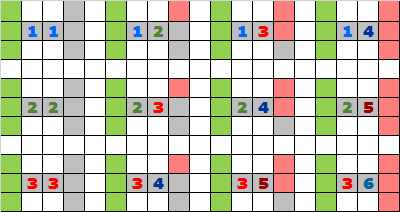
\includegraphics[scale=0.6]{game/定式1.png}
\end{center}
常用的111、1111、212、2112是相邻减法的推论。
\begin{center}
    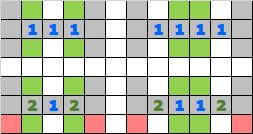
\includegraphics[scale=0.6]{game/定式6.png}
\end{center}

\vspace{5mm}对称减法(不完全举例):
\begin{center}
    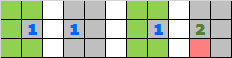
\includegraphics[scale=0.6]{game/定式2.png}
\end{center}

\vspace{5mm}121系列:
\begin{center}
    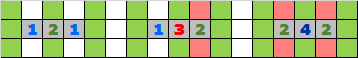
\includegraphics[scale=0.6]{game/定式3.png}
\end{center}

\vspace{5mm}变形的121系列:
\begin{center}
    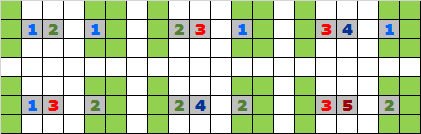
\includegraphics[scale=0.6]{game/定式4.png}
\end{center}
常用的1221定式是变形121的推论。
\begin{center}
    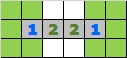
\includegraphics[scale=0.6]{game/定式7.png}
\end{center}

\vspace{5mm}角222、角131:
\begin{center}
    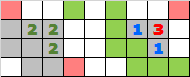
\includegraphics[scale=0.6]{game/定式5.png}
\end{center}
在竞速扫雷中,角222和角131的作用主要是把本来由两边共用的角处2或3拆分成在两边各1雷,从而可以应用其他定式。
\begin{center}
    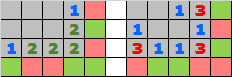
\includegraphics[scale=0.6]{game/定式8.png}
\end{center}
上左图中角222实际上在两边分别生成了121和1221定式。上右图中的三个角131实际上在两边分别生成了212和2112定式。

\subsection{挖坑}
挖坑实际上就是减法和连续减法的反复应用过程。这里给出挖坑时经常遇到的情况。挖坑重要的是方法而不是定式。

\vspace{5mm}平面、边缘挖坑:
\begin{center}
    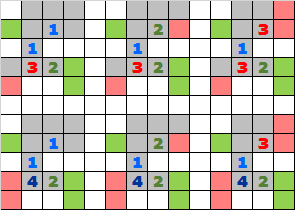
\includegraphics[scale=0.6]{game/挖坑1.png}
\end{center}

\vspace{5mm}拐角挖坑:
\begin{center}
    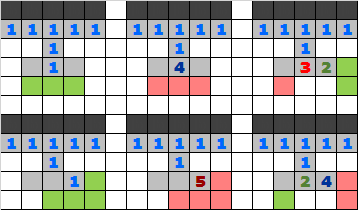
\includegraphics[scale=0.6]{game/挖坑2.png}
\end{center}

\subsection{环}\label{cycle}
环只会在中间开局时遇到。不等式可以解环。环的花样比挖坑更多,所以更需要掌握方法。

\vspace{5mm}
\begin{center}
    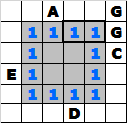
\includegraphics{trick/环1.png}
\end{center}
用黑框中的11做减法得到$A\ge C$。同理$C\ge D\ge E\ge A$,所以$A=C=D=E$。回到等式$A=C+G$,发现$G=0$。

\vspace{5mm}
\begin{center}
    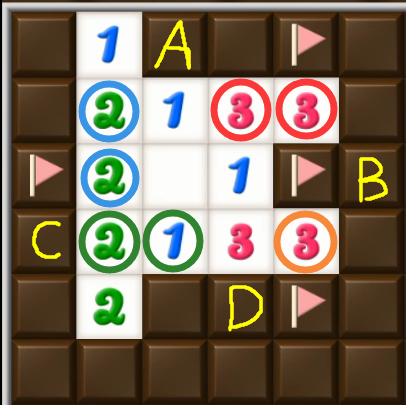
\includegraphics[width=0.5\textwidth]{trick/环2.png}
\end{center}
红圈33减法得$A\ge B$,蓝圈22减法得$C\ge A$,绿圈12减法得$D\ge C$,所以$D\ge B$。又因为橙圈3,$B+D\le 1$,所以$B=0$。

\vspace{5mm}
\begin{center}
    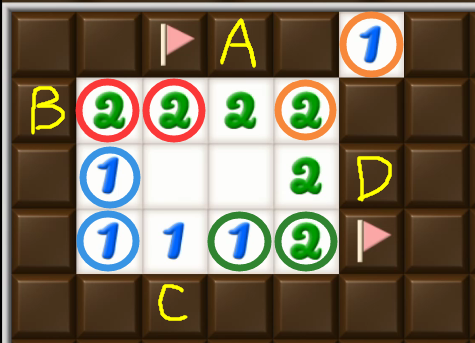
\includegraphics[width=0.5\textwidth]{trick/环3.png}
\end{center}
红圈22减法得$A\ge B$,蓝圈11减法得$B\ge C$,绿圈12减法得$C\ge D$,所以$A\ge D$。又用橙圈12减法得$A+D\ge 1$,所以$A=1$。

和连续减法类似,解环时一般不需要很小心地选取起始点,从很多地方开始都能得到等价的结论。读者可以尝试在上面两个例子中选择其他起始点生成连续不等式。下面就提供另一种起始方式。

\vspace{5mm}
\begin{center}
    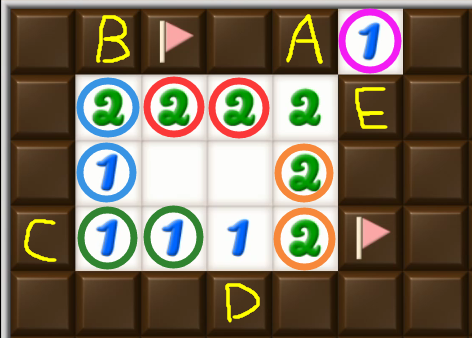
\includegraphics[width=0.5\textwidth]{trick/环4.png}
\end{center}
红圈22减法得$A=B$,蓝圈21减法得$C\ge B$,绿圈11减法得$D\ge C$,橙圈22减法得$E\ge D$,所以$E\ge A$。又因为粉圈1,$A+E\le 1$,所以$A=0$。

\vspace{5mm}
有时环不一定是方方正正的。只要逻辑上成环即可。

\vspace{5mm}
\begin{center}
    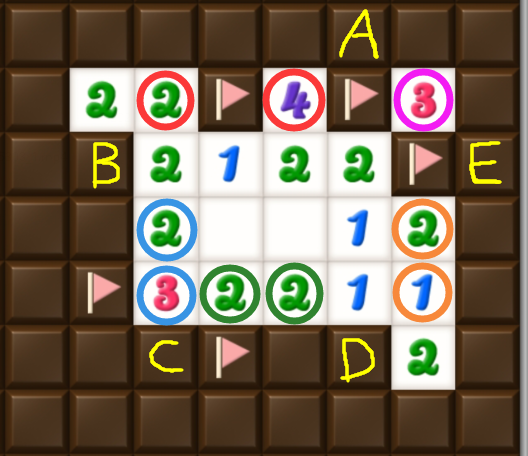
\includegraphics[width=0.5\textwidth]{trick/环5.png}
\end{center}
红圈42减法得$A\ge B$,蓝圈23减法得$B\ge C$,绿圈22减法得$C=D$,所以$A\ge D$。又由橙圈21减法得$E\ge D$,由粉圈3得$A+E\le 1$,所以$D=0$。

\vspace{5mm}
\begin{center}
    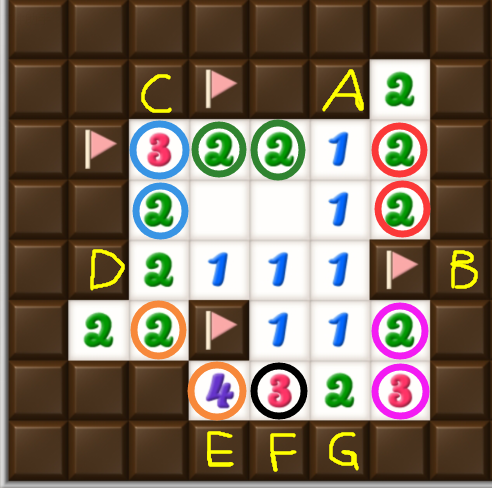
\includegraphics[width=0.5\textwidth]{trick/环6.png}
\end{center}
红圈22减法得$A\ge B$,绿圈22减法得$C\ge A$,蓝圈23减法得$D\ge C$,橙圈42减法得$E\ge D$且$F\ge D$,所以$E\ge B$且$F\ge B$。粉圈32减法得$G\ge B$。又因为黑圈3,$E+F+G=2$,所以$B=0$。

\vspace{5mm}
\begin{center}
    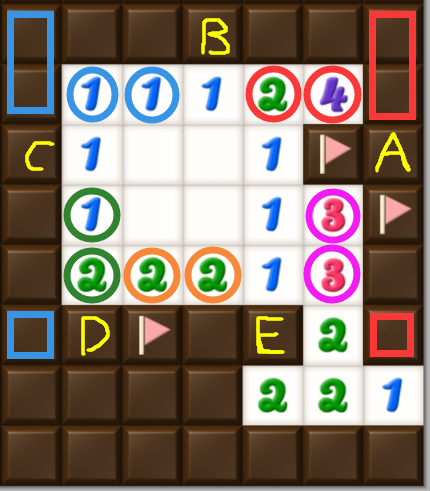
\includegraphics[width=0.5\textwidth]{trick/环7.png}
\end{center}
红圈42减法得$A\ge B$,蓝圈11减法得$B\ge C$,绿圈12减法得$C\ge D$,橙圈22减法得$D=E$,粉圈33减法得$E\ge A$,所以$A=B=C=D=E$。回顾用过的所有减法得红框为雷,蓝框安全。